\section{局部近似更新}
\label{sec:block-local}

精确块更新要求条件子问题便宜可解。许多目标不满足这一点，比如条件函数含对数或指数，每解一次都要内层迭代。这就需要回答：解不动条件子问题时，怎样在当前块上构造一个可以计算的局部模型，并用它推进完整目标？

三种模型对应三种读数。下表把它们和精确块更新放在一起比较。

\begin{BookInlineTable}
\centering
\begin{tabular}{p{20mm}p{24mm}p{22mm}p{22mm}}
\toprule
更新 & 每步读取 & 子问题 & 接受条件\\
\midrule
精确块解 & 条件函数 & 条件子问题 & 无需检验\\
BCGD & 当前点偏梯度 & 闭式的二次函数 & 步长$1/L_J$\\
APCG & 外推点偏梯度 & 闭式或邻近映射 & 无单调保证\\
块Newton & 偏梯度与块Hessian & 块内线性方程 & 线搜索等\\
\bottomrule
\end{tabular}
\end{BookInlineTable}

下面逐个看它们要解什么子问题、需要什么接受条件。

\subsection{块坐标梯度下降（BCGD）}
\label{sec:block-bcgd}

\paragraph{主要思想}
上一节的上界~\eqref{eq:block-quadratic-upper}是块$J$上的一个二次模型，它在当前点与$f$相等，并且处处不低于$f$。最小化这个上界代替最小化$f$，只走一步块梯度：
\begin{equation}
 \bm{x}_J^{(t+1)}=\bm{x}_J^{(t)}-\frac{1}{L_J}\nabla_Jf(\bm{x}^{(t)}),\qquad
 \bm{x}_i^{(t+1)}=\bm{x}_i^{(t)}\ \ (i\notin J).
 \label{eq:block-bcgd}
\end{equation}
这就是\term{块坐标梯度下降}（block coordinate gradient descent，BCGD）。由式~\eqref{eq:block-guaranteed-decrease}，每一步完整目标至少下降
\begin{equation}
 f(\bm{x}^{(t)})-f(\bm{x}^{(t+1)})\geq\frac{\lVert\nabla_Jf(\bm{x}^{(t)})\rVert_2^2}{2L_J}.
 \label{eq:block-bcgd-decrease}
\end{equation}

图~\ref{fig:block-upper-bound}(a)是一个不能闭式解出的条件函数$\varphi(z)=\sqrt{1+z^2}-z/2$，它的二阶导数不超过$1$，所以$L_J=1$。当前点$z=2$处$\varphi'(2)\approx0.394$，上界的最小点是$z^+=2-0.394=1.606$。上界（绿）紧贴在$\varphi$（蓝）的上方，上界的最小值高于真实函数在$z^+$处的值，所以真实下降量不会少于上界的下降量。

\begin{BookInlineFigure}
  \centering
  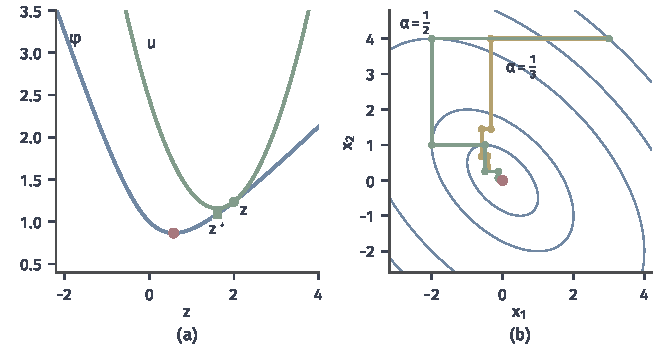
\includegraphics[width=112mm]{figures/05-optimization/04-block-optimization/matplotlib/block-upper-bound/figure.pdf}
  \caption{块梯度步的两个视角。(a)条件函数$\varphi(z)=\sqrt{1+z^2}-z/2$（蓝）与$L_J=1$的二次上界（绿），绿点是当前点$z=2$，空心点和方块分别是上界和原函数在上界最小点$z^+\approx1.606$处的值，红点是原函数的最小点$z\approx0.577$。(b)式~\eqref{eq:block-example}上循环BCGD的路径，绿色是块步长$\alpha=1/L_j=\tfrac12$，黄色是全局步长$\alpha=1/L=\tfrac13$，各画三轮。}
  \label{fig:block-upper-bound}
\end{BookInlineFigure}

\paragraph{块常数与全局常数}
最小二乘按样本数归一化时，目标是
\[
 f(\bm{x})=\frac{1}{2N}\lVert\bm{A}\bm{x}-\bm{b}\rVert_2^2 .
\]
坐标$j$的偏导数和块光滑常数是
\begin{equation}
 \partial_jf(\bm{x})=\frac{1}{N}\bm{a}_j^\top\bm{r},\qquad L_j=\frac{\lVert\bm{a}_j\rVert_2^2}{N},
 \label{eq:block-ls-constants}
\end{equation}
其中$\bm{r}=\bm{A}\bm{x}-\bm{b}$是残差。若目标不除以$N$，$L_j$和偏导数中的$1/N$同时去掉，步长与偏导数的乘积不变，所以两种写法走出的路径相同。块$J$含多列时，$L_J=\lambda_{\max}(\bm{A}_J^\top\bm{A}_J)/N$，其中$\bm{A}_J$是由这些列组成的子矩阵。

全局光滑常数是$L=\lambda_{\max}(\bm{A}^\top\bm{A})/N$。设$\bm{H}=\bm{A}^\top\bm{A}/N$半正定，每个对角元$L_j=\bm{e}_j^\top\bm{H}\bm{e}_j$不超过最大特征值，而最大特征值又不超过所有特征值之和，即迹。因此
\begin{equation}
 L_j\leq L\leq\sum_{i=1}^nL_i .
 \label{eq:block-constant-order}
\end{equation}

式~\eqref{eq:block-constant-order}的左半边解释了坐标法为什么敢走得更远：上界只要在这一个方向上成立，曲率只需按这一方向计算，而全局步长必须照顾最陡的方向。列相关性很强时$L$可接近$\sum_iL_i$，坐标步长可以比全局步长大$n$倍。

例中$\bm{A}$的两列平方范数都是$2$，未归一化时
\[
 L_1=L_2=2,\qquad L=\lambda_{\max}(\bm{Q})=3 .
\]
块步长是$\tfrac12$，全局步长是$\tfrac13$。图~\ref{fig:block-upper-bound}(b)比较了这两种步长：步长$\tfrac13$的每一阶都没有走到条件最小点，路径的收缩更慢。

\needspace{6\baselineskip}
\paragraph{变量}
\begin{itemize}
 \item $\bm{x}\in\mathbb{R}^n$：当前点。
 \item $\bm{r}=\bm{A}\bm{x}-\bm{b}\in\mathbb{R}^N$：维护的残差，读偏导数时使用。
 \item $L_j$：各坐标的块光滑常数，事先算好。
\end{itemize}

\paragraph{初始化}
算出各$L_j$和初始残差$\bm{r}^{(0)}$，令$t=0$。例中用$\bm{A}$的三行，$\bm{b}=\bm{0}$，$\bm{x}^{(0)}=(3,4)$，不除以$N$：
\[
 L_1=L_2=2,\qquad \bm{r}^{(0)}=\bm{A}\bm{x}^{(0)}=(7,3,4).
\]

\needspace{6\baselineskip}
\paragraph{每轮更新}
按某个选块规则取坐标$j$，然后：
\begin{enumerate}
 \item \textbf{读偏导数。}计算$\partial_jf=\bm{a}_j^\top\bm{r}$。例中第一轮先取$j=1$，
 \[
  \partial_1f=7+3=10 .
 \]
 \item \textbf{更新变量。}由式~\eqref{eq:block-bcgd}，位移是$\delta=-\partial_jf/L_j$，令$x_j\leftarrow x_j+\delta$。例中
 \[
  \delta=-5,\qquad x_1=-2 .
 \]
 \item \textbf{更新残差。}令$\bm{r}\leftarrow\bm{r}+\delta\bm{a}_j$，不重算矩阵乘向量。例中
 \[
  \bm{r}=(7,3,4)-5(1,1,0)=(2,-2,4).
 \]

 例中第一轮再取$j=2$，$\partial_2f=2+4=6$，$\delta=-3$，于是
 \[
  x_2=1,\qquad \bm{r}=(2,-2,4)-3(1,0,1)=(-1,-2,1).
 \]
 此时目标值是$\tfrac12\lVert\bm{r}\rVert_2^2=3$。

 例中第二轮取$j=1$，$\partial_1f=-3$，$\delta=\tfrac32$，于是
 \[
  x_1=-\tfrac12,\qquad \bm{r}=\bigl(\tfrac12,-\tfrac12,1\bigr).
 \]

 再取$j=2$，$\partial_2f=\tfrac32$，$\delta=-\tfrac34$，于是
 \[
  x_2=\tfrac14,\qquad \bm{r}=\bigl(-\tfrac14,-\tfrac12,\tfrac14\bigr).
 \]
 此时目标值是$\tfrac{3}{16}$。
\end{enumerate}

迭代结束的条件与第~\ref{sec:block-cyclic}小节相同。最终得到的点和循环精确更新完全一致，第$t$轮结束时都是$\bm{x}^{(t)}=(-2\cdot4^{1-t},4^{1-t})$。原因是二次目标的条件函数本身就是抛物线，上界~\eqref{eq:block-quadratic-upper}取$L_j=Q_{j,j}$时恰好等于条件函数，上界的最小点就是条件最小点。对一般光滑目标，两种更新不同。

\subsection{加速邻近坐标梯度（APCG）}
\label{sec:block-apcg}

\paragraph{要解决的问题}
BCGD每步只用当前点的信息，和梯度下降一样没有利用走过的路。第~\ref{chap:first-order-methods}章的加速方法靠外推把凸目标的目标差从$O(1/t)$提到$O(1/t^2)$，自然想把同样的思想用在坐标更新上。\term{加速邻近坐标梯度}（accelerated proximal coordinate gradient，APCG）方法就做这件事，并且允许目标含按块可分的非光滑项。

考虑
\begin{equation}
 \min_{\bm{x}\in\mathbb{R}^n}\ F(\bm{x})=f(\bm{x})+\sum_{J}g_J(\bm{x}_J),
 \label{eq:block-composite}
\end{equation}
其中$f$是凸函数，关于每一块满足定义~\ref{def:block-smooth}，每个$g_J$是适当、闭的凸函数。回顾第~\ref{chap:nonsmooth-composite-optimization}章的邻近映射
\[
 \operatorname{prox}_{\alpha g}(\bm{v})=\argmin_{\bm{u}}\Bigl\{g(\bm{u})+\frac{1}{2\alpha}\lVert\bm{u}-\bm{v}\rVert_2^2\Bigr\},
\]
它把“沿梯度走一步”之后的点拉回到非光滑项喜欢的位置，$g\equiv0$时就是恒等映射。

\paragraph{三条序列}
APCG维护三条序列，图~\ref{fig:block-apcg-sequences}是它们的关系。$\bm{x}^{(t)}$是报告给用户的点；$\bm{z}^{(t)}$记录累积的梯度信息，每次走较长的步子；$\bm{y}^{(t)}$是这两者的组合，只在这一点上读偏梯度。

\begin{BookInlineFigure}
  \centering
  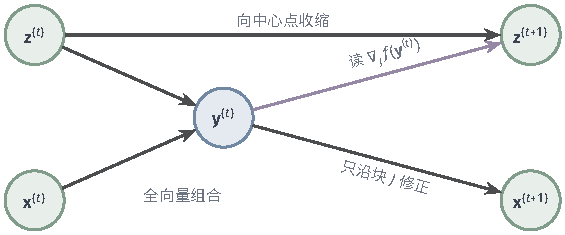
\includegraphics[width=95mm]{figures/05-optimization/04-block-optimization/tikz/block-apcg-sequences/figure.pdf}
  \caption{APCG一步中三条序列的依赖关系。$\bm{y}^{(t)}$是$\bm{x}^{(t)}$与$\bm{z}^{(t)}$的组合，这一步通常改变全部分量；在$\bm{y}^{(t)}$处读抽中块$J$的偏梯度（紫色）后，$\bm{z}$沿块$J$走一长步，$\bm{x}^{(t+1)}$只在$\bm{y}^{(t)}$的块$J$上修正一步。}
  \label{fig:block-apcg-sequences}
\end{BookInlineFigure}

为什么$\bm{z}$的步长要放大？一次只抽一块，每一块平均$B$步才轮到一次。$\bm{z}$是积累全局信息的序列，它要把偶尔读到的这一块的信息放大，才能代表整个梯度的作用，所以步长是$1/L_J$的$1/(B\alpha^{(t)})$倍。$\bm{x}$只负责走稳妥的短步。这和第~\ref{chap:first-order-methods}章的外推相似：先在外推点读梯度，再决定位移。不同的是，这里的读数只有一块，$\bm{z}$的放大倍数正是用来补偿这一点的。

分析中用到按块常数加权的范数
\begin{equation}
 \lVert\bm{x}\rVert_L^2=\sum_{J}L_J\lVert\bm{x}_J\rVert_2^2 .
 \label{eq:block-L-norm}
\end{equation}
设$f$关于这个范数有强凸常数$\mu_L\geq0$，也就是说，对任意$\bm{x},\bm{y}$，
\[
 f(\bm{y})\geq f(\bm{x})+\langle\nabla f(\bm{x}),\bm{y}-\bm{x}\rangle+\frac{\mu_L}{2}\lVert\bm{y}-\bm{x}\rVert_L^2 .
\]
$\mu_L=0$表示只要求凸。这样定义的$\mu_L$不超过$1$，因为沿块方向它受块光滑常数限制。

\paragraph{迭代公式}
记$B$为块数，选$\gamma^{(0)}\in[\mu_L,1]$且$\gamma^{(0)}>0$，令$\bm{z}^{(0)}=\bm{x}^{(0)}$。第$t$步先由下面的方程取$\alpha^{(t)}\in(0,1/B]$，并更新另外两个参数：
\begin{equation}
 \begin{gathered}
 B^2(\alpha^{(t)})^2=(1-\alpha^{(t)})\gamma^{(t)}+\alpha^{(t)}\mu_L,\\
 \gamma^{(t+1)}=B^2(\alpha^{(t)})^2,\qquad
 \beta^{(t)}=\frac{\alpha^{(t)}\mu_L}{\gamma^{(t+1)}} .
 \end{gathered}
 \label{eq:block-apcg-params}
\end{equation}
然后构造外推点和$\bm{z}$的中心点：
\begin{equation}
 \begin{aligned}
 \bm{y}^{(t)}&=\frac{\alpha^{(t)}\gamma^{(t)}\bm{z}^{(t)}+\gamma^{(t+1)}\bm{x}^{(t)}}{\alpha^{(t)}\gamma^{(t)}+\gamma^{(t+1)}},\\
 \bm{w}^{(t)}&=(1-\beta^{(t)})\bm{z}^{(t)}+\beta^{(t)}\bm{y}^{(t)} .
 \end{aligned}
 \label{eq:block-apcg-extrapolate}
\end{equation}

独立均匀地抽一块$J$，在$\bm{y}^{(t)}$处读偏梯度。记$\tau=1/(B\alpha^{(t)}L_J)$，这是比$1/L_J$更长的步长。块$J$上用邻近步更新$\bm{z}$，其余块取中心点的值：
\begin{equation}
 \bm{z}_J^{(t+1)}=\operatorname{prox}_{\tau g_J}\bigl(\bm{w}_J^{(t)}-\tau\nabla_Jf(\bm{y}^{(t)})\bigr),\qquad
 \bm{z}_i^{(t+1)}=\bm{w}_i^{(t)}\ \ (i\notin J).
 \label{eq:block-apcg-z}
\end{equation}
最后由$\bm{y}$和$\bm{z}$的变化得到新迭代点：
\begin{equation}
 \bm{x}^{(t+1)}=\bm{y}^{(t)}+B\alpha^{(t)}\bigl(\bm{z}^{(t+1)}-\bm{w}^{(t)}\bigr).
 \label{eq:block-apcg-x}
\end{equation}

式~\eqref{eq:block-apcg-z}中$\bm{z}^{(t+1)}$和$\bm{w}^{(t)}$只在块$J$上不同，所以$\bm{x}^{(t+1)}$相对$\bm{y}^{(t)}$也只改变块$J$。$g_J\equiv0$时，代入式~\eqref{eq:block-apcg-x}，块$J$上得到
\[
 \bm{x}_J^{(t+1)}=\bm{y}_J^{(t)}-\frac{1}{L_J}\nabla_Jf(\bm{y}^{(t)}),
\]
这正是在外推点上的一步BCGD。外推本身却可能改变全向量，这是加速方法计算上的主要负担，下文计入成本。

\needspace{6\baselineskip}
\paragraph{变量}
\begin{itemize}
 \item $\bm{x}^{(t)},\bm{z}^{(t)}\in\mathbb{R}^n$：报告点和累积序列。
 \item $\bm{y}^{(t)},\bm{w}^{(t)}\in\mathbb{R}^n$：外推点和$\bm{z}$的中心点，每步由前两者算出。
 \item $\alpha^{(t)},\beta^{(t)},\gamma^{(t)}$：由式~\eqref{eq:block-apcg-params}确定的标量。
\end{itemize}

\paragraph{初始化}
令$\bm{z}^{(0)}=\bm{x}^{(0)}$，选$\gamma^{(0)}$。取$\gamma^{(0)}=\mu_L>0$时，由式~\eqref{eq:block-apcg-params}可知各参数不随$t$变化：
\[
 \gamma^{(t)}=\mu_L,\qquad \alpha^{(t)}=\beta^{(t)}=\frac{\sqrt{\mu_L}}{B}.
\]

例中为了得到整齐的参数，把交叉项系数改成$c=\tfrac32$，即用$f_{3/2}$，$B=2$。此时$L_1=L_2=2$，$\lVert\bm{x}\rVert_L^2=2\lVert\bm{x}\rVert_2^2$，Hessian的最小特征值是$\tfrac12$，于是
\[
 \mu_L=\frac14,\qquad \alpha^{(t)}=\beta^{(t)}=\frac14 .
\]
起点仍取$\bm{x}^{(0)}=\bm{z}^{(0)}=(3,4)$，目标值$f=43$。$g_J\equiv0$，步长$\tau=1/(2\cdot\tfrac14\cdot2)=1$。

\needspace{6\baselineskip}
\paragraph{每轮更新}
第$t$步依次做：
\begin{enumerate}
 \item \textbf{外推。}按式~\eqref{eq:block-apcg-extrapolate}算$\bm{y}^{(t)}$和$\bm{w}^{(t)}$。例中公式化为
 \[
  \bm{y}=\frac{4\bm{x}+\bm{z}}{5},\qquad \bm{w}=\frac34\bm{z}+\frac14\bm{y}.
 \]
 第一步$\bm{x}=\bm{z}$，所以$\bm{y}=\bm{w}=(3,4)$。
 \item \textbf{抽块并读偏梯度。}例中第一步设抽到块$1$，
 \[
  \partial_1f(\bm{y})=2\cdot3+\tfrac32\cdot4=12 .
 \]
 \item \textbf{更新$\bm{z}$。}按式~\eqref{eq:block-apcg-z}。例中$\tau=1$，块$J$上$\bm{z}_J^{+}=\bm{w}_J-\nabla_Jf(\bm{y})$，第一步
 \[
  \bm{z}^{(1)}=(-9,4).
 \]
 \item \textbf{更新$\bm{x}$。}按式~\eqref{eq:block-apcg-x}。例中块$J$上$\bm{x}_J^{+}=\bm{y}_J-\tfrac12\nabla_Jf(\bm{y})$，第一步
 \[
  \bm{x}^{(1)}=(-3,4),\qquad f(\bm{x}^{(1)})=7 .
 \]

 例中第二步设抽到块$2$。先算外推点和中心点，
 \[
  \bm{y}=(-4.2,\,4),\qquad \bm{w}=(-7.8,\,4).
 \]
 偏导数$\partial_2f(\bm{y})=\tfrac32(-4.2)+8=1.7$，于是
 \[
  \bm{z}^{(2)}=(-7.8,\,2.3),\qquad \bm{x}^{(2)}=(-4.2,\,3.15),\qquad f(\bm{x}^{(2)})=7.7175 .
 \]

 例中第三步设抽到块$1$，同样计算得
 \[
  \bm{y}=(-4.92,\,2.98),\qquad \bm{w}=(-7.08,\,2.47),\qquad \partial_1f(\bm{y})=-5.37 ,
 \]
 于是
 \[
  \bm{z}^{(3)}=(-1.71,\,2.47),\qquad \bm{x}^{(3)}=(-2.235,\,2.98),\qquad f(\bm{x}^{(3)})=3.885175 .
 \]
\end{enumerate}

第二步的目标值从$7$升到了$7.7175$，这不是计算错误。APCG在外推点上读偏梯度，$\bm{x}^{(t+1)}$相对$\bm{y}^{(t)}$有下降保证，相对$\bm{x}^{(t)}$却没有，目标值不是单调的。迭代持续到外部设定的更新次数或目标差估计达到要求为止，图~\ref{fig:block-apcg-rate}(b)是继续迭代的结果。

\paragraph{收敛结论}
下面的结论把成立所需的条件都列了出来。证明要构造随机的估计序列，并逐步跟踪参数$\alpha^{(t)},\gamma^{(t)}$的递推，篇幅较长，读者可查阅Lin、Lu和Xiao关于APCG方法的原始论文。

\begin{theorem}[APCG的收敛率]
\label{thm:block-apcg}
设问题~\eqref{eq:block-composite}的解集非空，$f$是凸函数，满足定义~\ref{def:block-smooth}（全空间上成立），且关于范数~\eqref{eq:block-L-norm}的强凸常数为$\mu_L\geq0$；每个$g_J$是适当、闭的凸函数，邻近子问题~\eqref{eq:block-apcg-z}精确求解。设每步独立均匀地抽块，参数按式~\eqref{eq:block-apcg-params}取，$\gamma^{(0)}\in[\mu_L,1]$，$\gamma^{(0)}>0$。记$R_0=\min\lVert\bm{x}^{(0)}-\bm{x}^\star\rVert_L$，最小值取遍所有最优解。则对一切$t\geq0$，
\begin{equation}
 \mathbb{E}\bigl[F(\bm{x}^{(t)})\bigr]-F^\star\leq
 \min\Bigl\{\Bigl(1-\frac{\sqrt{\mu_L}}{B}\Bigr)^{t},\ \Bigl(\frac{2B}{2B+t\sqrt{\gamma^{(0)}}}\Bigr)^{2}\Bigr\}\,E_0,
 \label{eq:block-apcg-rate}
\end{equation}
其中
\begin{equation}
 E_0=F(\bm{x}^{(0)})-F^\star+\frac{\gamma^{(0)}}{2}R_0^2 .
 \label{eq:block-apcg-e0}
\end{equation}
\end{theorem}

这个结论有三层含义。$\mu_L=0$时，第二项给出$O(B^2/t^2)$的期望目标差，$t$次更新相当于$t/B$轮，所以按轮数算是$O(1/(t/B)^2)$，这是加速率。$\mu_L>0$且取$\gamma^{(0)}=\mu_L$时，第一项给出线性率，因子是$1-\sqrt{\mu_L}/B$，而第~\ref{sec:block-convergence}小节的BCGD因子相当于$1-\mu_L/B$，根号带来的差别在$\mu_L$很小时才明显。

例中$\mu_L=\tfrac14$，$B=2$，所以APCG的因子是$1-\tfrac14=\tfrac34$，BCGD的因子是$1-\tfrac18=\tfrac78$。定理保证的都是期望，并要求块是独立均匀抽取的，单次运行的路径可能波动。

条件的作用值得逐条看。块光滑常数给出沿块的二次上界，步长由它决定；精确的块邻近求解让加速递推的不等式能闭合，若解得不准，误差会在递推中累积，第~\ref{sec:block-inexact}小节讨论的误差控制不能直接搬过来；解的存在保证$R_0$有限，否则右端没有意义。

图~\ref{fig:block-apcg-rate}显示了加速的效果和代价。(a)是链式二次目标，没有可用的强凸常数，APCG（绿）的目标差贴着虚线$t^{-2}$下降，明显快于BCGD（黄）。(b)是手算例子的延续，APCG整体更快，但曲线有回升。

\begin{BookInlineFigure}
  \centering
  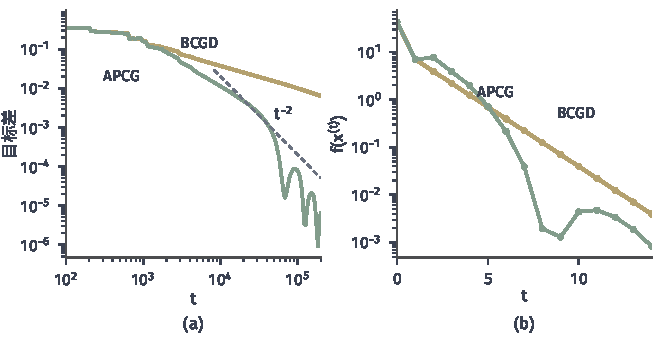
\includegraphics[width=112mm]{figures/05-optimization/04-block-optimization/matplotlib/block-apcg-rate/figure.pdf}
  \caption{APCG的数值表现。(a)链式二次目标，$n=200$，单坐标块，绿线是APCG（$\mu_L=0$），黄线是BCGD，都是$4$次独立运行的平均，灰色虚线是斜率为$-2$的参考线。(b)$f_{3/2}$从$(3,4)$出发，按块$1,2,1,2,\ldots$的顺序，绿线是APCG（$\alpha^{(t)}=\beta^{(t)}=\tfrac14$），黄线是步长$\tfrac12$的BCGD，APCG的目标值并不单调。}
  \label{fig:block-apcg-rate}
\end{BookInlineFigure}

\paragraph{计算成本}
一步APCG除了读一个偏梯度，还要做式~\eqref{eq:block-apcg-extrapolate}这样的全向量组合，直接实现的代价是$O(n)$，可能抵消单坐标更新省下的计算。实现时可以把$\bm{x},\bm{z}$写成两个基向量的线性组合，组合系数是标量，每步只更新基向量的一块，外推就不必真正展开。

偏梯度读取仍然需要在$\bm{y}^{(t)}$处求值。对最小二乘，维护$\bm{A}$作用在两个基向量上的结果即可，每步成本和BCGD同量级。这一点依赖目标的结构；$\nabla_Jf$不能增量维护时，一步的成本仍是$O(n)$或更高。

\subsection{块坐标Newton法}
\label{sec:block-newton}

\paragraph{主要思想}
块梯度步只用一阶信息，块内变量强耦合时，它和全局梯度下降一样走折线。第~\ref{chap:second-order-methods}章用Hessian修正方向，这里只对当前块做同样的事。设$f$二阶连续可微，把二阶Taylor模型限制在块$J$上：
\[
 m_J(\bm{h})=f(\bm{x})+\langle\nabla_Jf(\bm{x}),\bm{h}\rangle+\frac12\bm{h}^\top\bm{H}_{J,J}\bm{h},
\]
其中$\bm{H}_{J,J}$是Hessian的块$J$主子矩阵，即
\[
 \bm{H}_{J,J}=\bm{U}_J^\top\nabla^2f(\bm{x})\bm{U}_J .
\]
$\bm{H}_{J,J}$正定时模型有唯一最小点，得到块Newton方向：
\begin{equation}
 \bm{d}_J=-\bm{H}_{J,J}^{-1}\nabla_Jf(\bm{x}).
 \label{eq:block-newton}
\end{equation}
\term{块坐标Newton法}（block coordinate Newton method）沿这个方向更新块$J$，其余块不动。

\paragraph{正定性、修正与阻尼}
第~\ref{chap:second-order-methods}章对完整Newton法提出的三个问题，在这里同样存在，只是规模换成了块。第一是正定性：若$\nabla^2f(\bm{x})$正定，它的任何主子矩阵也正定，并且最小特征值不小于$\nabla^2f(\bm{x})$的最小特征值，块方向总是下降方向。

非凸目标的$\bm{H}_{J,J}$可能不定，这时要加修正，比如把它换成$\bm{H}_{J,J}+\tau\bm{I}$。第二是步长：二阶模型只是局部近似，不保证$\bm{d}_J$上目标下降，需要沿该方向回溯，令$\bm{x}_J^{+}=\bm{x}_J+\alpha\bm{d}_J$，用完整目标检验$\alpha$是否可接受。第三是成本：下面单独计算。

\paragraph{何时等于精确块解}
二次目标的$\bm{H}_{J,J}$是常数$\bm{Q}_{J,J}$，二阶模型恰好等于条件函数。令$\bm{d}_J$由式~\eqref{eq:block-newton}给出，$\bm{x}_J+\bm{d}_J$就是式~\eqref{eq:block-quadratic-solve}的精确块解。

例中$J=\{1\}$，点$(3,4)$处$\partial_1f=10$，$H_{1,1}=2$，方向$d_1=-5$，新值$x_1=-2$，和精确块解相同。

一般的非线性目标则不同。设条件函数是$\varphi(z)=z^4+2z$，当前$z=1$，则
\[
 \varphi'(1)=6,\qquad\varphi''(1)=12,\qquad z^{+}=1-\frac{6}{12}=0.5 .
\]
而精确块解满足$4z^3+2=0$，即$z\approx-0.794$，两者差很远。Newton步解的是模型，只有模型足够准确时才接近精确块解。图~\ref{fig:block-newton-slice}对比了这两种情形。

\begin{BookInlineFigure}
  \centering
  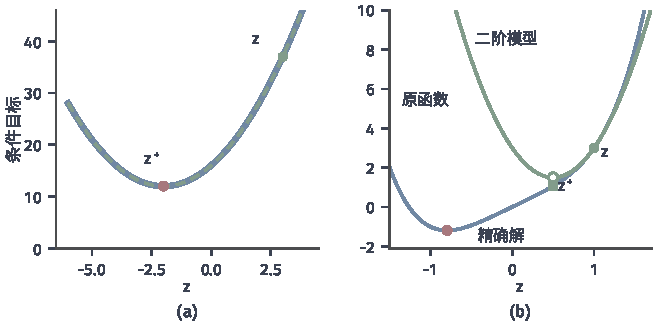
\includegraphics[width=112mm]{figures/05-optimization/04-block-optimization/matplotlib/block-newton-slice/figure.pdf}
  \caption{块Newton步与精确块解。(a)二次条件函数$\varphi(z)=z^2+4z+16$，蓝色实线与绿色虚线分别是原函数和二阶模型，两者重合，Newton步一步到达条件最小点。(b)非二次条件函数$\varphi(z)=z^4+2z$在$z=1$处，绿色的二阶模型只在附近贴近原函数（蓝），它的最小点$z^+=0.5$（空心点）与原函数的最小点（红）相距较远。}
  \label{fig:block-newton-slice}
\end{BookInlineFigure}

\paragraph{成本}
块大小$p=\lvert J\rvert$时，一步块Newton需要形成$\bm{H}_{J,J}$的$O(p^2)$个元素，并以约$p^3/3$的运算量做Cholesky分解。固定其他块时若$\bm{H}_{J,J}$不变，分解可以复用，这在二次目标上正是图~\ref{fig:block-size-cost}的成本模型；一般非线性目标的Hessian随迭代变化，分解要反复计算。
